%%%%%%%%%%%%%%%%%%%%%%%%%%%%%%%%%%%%%%%%%%%%%%%%%%%%%%%%%%%%%%%%%%%%%%%%%%%%%%%
% Chapter 'Absorption - CarbonDioxide - ionic liquid [N4,1,1,1][NTf2]'
%%%%%%%%%%%%%%%%%%%%%%%%%%%%%%%%%%%%%%%%%%%%%%%%%%%%%%%%%%%%%%%%%%%%%%%%%%%%%%%
\subsection{Ionic liquid [N4,1,1,1][NTf2]}
%
%%%%%%%%%%%%%%%%%%%%%%%%%%%%%%%%%%%%%%%%%%%%%%%%%%%%%%%%%%%%%%%%%%%%%%%%%%%%%%%
%%%%%%%%%%%%%%%%%%%%%%%%%%%%%%%%%%%%%%%%%%%%%%%%%%%%%%%%%%%%%%%%%%%%%%%%%%%%%%%
\subsubsection{MixingRule - ID 1}
%
\begin{tabular}[l]{|lp{11.5cm}|}
\hline
\addlinespace

\textbf{Sorbent:} & ionic liquid \\
\textbf{Subtype:} & [N4,1,1,1][NTf2] \\
\textbf{Refrigerant:} & CarbonDioxide \\
\textbf{Equation:} & MixingRule \\
\textbf{ID:} & 1 \\
\textbf{Reference:} & Manic, Marina S.; Queimada, António J.; Macedo, Eugénia A.; Najdanovic-Visak, Vesna (2012): High-pressure solubilities of carbon dioxide in ionic liquids based on bis(trifluoromethylsulfonyl)imide and chloride. In: The Journal of Supercritical Fluids 65, S. 1–10. DOI: 10.1016/j.supflu.2012.02.016. \\
\textbf{Comment:} & None \\

\addlinespace
\hline
\end{tabular}
\newline

\textbf{Equation and parameters:}
\newline
%
Vapor pressure $p_\mathrm{sat}$ in $\si{\pascal}$ is calculated depending on temperature $T$ in $\si{\kelvin}$ and molar volume v in $\si{\mole\per\cubic\meter}$ by using cubic equation of state. For this purpose, molar volumes of liquid and vapor phase are changed iteratively until fugacity coefficients of vapor and liquid phase are equal. Cubic equation of state and mixing rules are given by:
\begin{equation*}
\begin{split}
p &=& R \frac{T}{v - b} - \frac{a}{v \left(v + b\right) + b \left(v - b\right)} & \quad\text{, and} \\
a &=& z_1^2 a_1 + 2 z_1 z_2 a_{12} + 2_2^2 a_2 & \quad\text{, and} \\
b &=& z_1 b_1 + z_2 b_2 & \quad\text{, and} \\
a_{12} &=& \left( a_1 a_2 \right) ^{0.5} \left(1 - k_{12} \right) & \quad\text{, and} \\
z_j &=& x_j \textrm { or } y_j \textrm{ depending on phase} & \quad\text{, and} \\
a_j &=& 0.45724 \frac{\left(R T_{\mathrm{crit},j} \right)^2}{p_{\mathrm{crit},j}} \alpha_j & \quad\text{, and} \\
b_j &=& 0.07780 R \frac{T_{\mathrm{crit},j}}{p_{\mathrm{crit},j}} & \quad\text{, and} \\
\alpha_j &=& \left(1 + \kappa_j \left(1 - \sqrt(\nicefrac{T}{T_{\mathrm{crit},j}}) \right) \right)^2 & \quad\text{, and} \\
\kappa_j &=& 0.37464 + 1.54226 \omega_j - 0.26992 \omega_j^2 & \quad\text{.}
\end{split}
\end{equation*}
%
The parameters of the equation are:
%
\begin{longtable}[l]{lll|lll}
\toprule
\addlinespace
\textbf{Par.} & \textbf{Unit} & \textbf{Value} &	\textbf{Par.} & \textbf{Unit} & \textbf{Value} \\
\addlinespace
\midrule
\endhead

\bottomrule
\endfoot
\bottomrule
\endlastfoot
\addlinespace

EoS & - & 1.000000000e+01 & Mix & - & -5.000000000e+00 \\
$T_\mathrm{crit,1}$ & $\si{\kelvin}$ & 3.042000000e+02 & $T_\mathrm{crit,2}$ & $\si{\kelvin}$ & 1.079600000e+03 \\
$p_\mathrm{crit,1}$ & $\si{\pascal}$ & 7.380000000e+06 & $p_\mathrm{crit,2}$ & $\si{\pascal}$ & 2.588000000e+06 \\
$\omega_{1}$ & - & 2.236000000e-01 & $\omega_{2}$ & - & 3.334000000e-01 \\
$\kappa_{1,1}$ & - & 0.000000000e+00 & $\kappa_{1,2}$ & - & 0.000000000e+00 \\
$\beta_{0,1}$ & - & 0.000000000e+00 & $\beta_{0,2}$ & - & 0.000000000e+00 \\
$\beta_{1,1}$ & - & 0.000000000e+00 & $\beta_{1,2}$ & - & 0.000000000e+00 \\
$\beta_{2,1}$ & - & 0.000000000e+00 & $\beta_{2,2}$ & - & 0.000000000e+00 \\
$\beta_{3,1}$ & - & 0.000000000e+00 & $\beta_{3,2}$ & - & 0.000000000e+00 \\
$k_{12}$ & - & -6.000000000e-04 & $m$ & - & 0.000000000e+00 \\
$l_{12}$ & - & 0.000000000e+00 & $l_{21}$ & - & 0.000000000e+00 \\
$t$ & - & 0.000000000e+00 & & & \\

\addlinespace\end{longtable}

\textbf{Validity:}
\newline
Equation is approximately valid for $313.15 \si{\kelvin} \leq T \leq 323.15 \si{\kelvin}$.
\newline

\textbf{Visualization:}
%
\begin{figure}[!htp]
{\noindent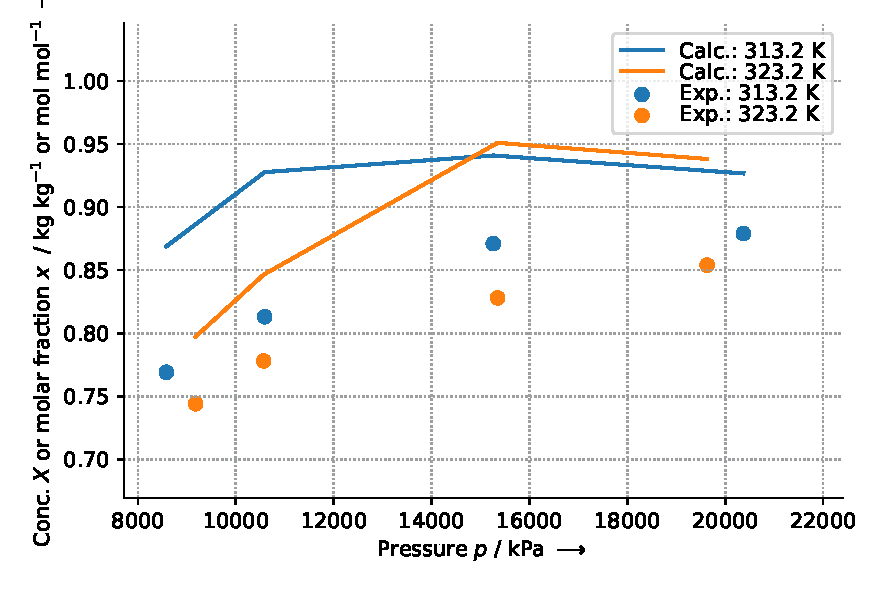
\includegraphics[height=10cm, keepaspectratio]{figs/abs/abs_CarbonDioxide_ionic_liquid_[N4,1,1,1][NTf2]_MixingRule_1.pdf}}
\end{figure}
%

To generate the figure, the following refrigerant functions were selected:
\begin{itemize}
\item Vapor pressure: VaporPressure\_EoS1 - ID 1
\item Saturated liquid density: SaturatedLiquidDensity\_EoS1 - ID 1
\end{itemize}

The uncertainity of the experimental data is:
\begin{itemize}
\item Data source $\,\to\,$ Data was taken from table
\item Pressure, absolute, in $\si{\pascal}$ $\,\to\,$ 7.00E+03
\item Temperature, absolute, in $\si{\kelvin}$ $\,\to\,$ 0.1
\end{itemize}

The mean absolute percentage error (MAPE) between the experimental and calculated data results in 10.15\%.
\FloatBarrier
\newpage
%%%%%%%%%%%%%%%%%%%%%%%%%%%%%%%%%%%%%%%%%%%%%%%%%%%%%%%%%%%%%%%%%%%%%%%%%%%%%%%
%%%%%%%%%%%%%%%%%%%%%%%%%%%%%%%%%%%%%%%%%%%%%%%%%%%%%%%%%%%%%%%%%%%%%%%%%%%%%%%
\subsubsection{MixingRule - ID 2}
%
\begin{tabular}[l]{|lp{11.5cm}|}
\hline
\addlinespace

\textbf{Sorbent:} & ionic liquid \\
\textbf{Subtype:} & [N4,1,1,1][NTf2] \\
\textbf{Refrigerant:} & CarbonDioxide \\
\textbf{Equation:} & MixingRule \\
\textbf{ID:} & 2 \\
\textbf{Reference:} & Manic, Marina S.; Queimada, António J.; Macedo, Eugénia A.; Najdanovic-Visak, Vesna (2012): High-pressure solubilities of carbon dioxide in ionic liquids based on bis(trifluoromethylsulfonyl)imide and chloride. In: The Journal of Supercritical Fluids 65, S. 1–10. DOI: 10.1016/j.supflu.2012.02.016. \\
\textbf{Comment:} & None \\

\addlinespace
\hline
\end{tabular}
\newline

\textbf{Equation and parameters:}
\newline
%
Vapor pressure $p_\mathrm{sat}$ in $\si{\pascal}$ is calculated depending on temperature $T$ in $\si{\kelvin}$ and molar volume v in $\si{\mole\per\cubic\meter}$ by using cubic equation of state. For this purpose, molar volumes of liquid and vapor phase are changed iteratively until fugacity coefficients of vapor and liquid phase are equal. Cubic equation of state and mixing rules are given by:
\begin{equation*}
\begin{split}
p &=& R \frac{T}{v - b} - \frac{a}{v \left(v + b\right)} & \quad\text{, and} \\
a &=& z_1^2 a_1 + 2 z_1 z_2 a_{12} + 2_2^2 a_2 & \quad\text{, and} \\
b &=& z_1 b_1 + z_2 b_2 & \quad\text{, and} \\
a_{12} &=& \left( a_1 a_2 \right) ^{0.5} \left(1 - k_{12} \right) & \quad\text{, and} \\
z_j &=& x_j \textrm { or } y_j \textrm{ depending on phase} & \quad\text{, and} \\
a_j &=& \frac{1}{9 \left(2^{\nicefrac{1}{3}} - 1\right)} \frac{\left(R T_{\mathrm{crit},j} \right)^2}{p_{\mathrm{crit},j}} \alpha_j & \quad\text{, and} \\
b_j &=& 0.08664 R \frac{T_{\mathrm{crit},j}}{p_{\mathrm{crit},j}} & \quad\text{, and} \\
\alpha_j &=& \left(1 + \kappa_j \left(1 - \sqrt(\nicefrac{T}{T_{\mathrm{crit},j}}) \right) \right)^2 & \quad\text{, and} \\
\kappa_j &=& 0.48508 + 1.55171 \omega_j - 0.15613 \omega_j^2 & \quad\text{.}
\end{split}
\end{equation*}
%
The parameters of the equation are:
%
\begin{longtable}[l]{lll|lll}
\toprule
\addlinespace
\textbf{Par.} & \textbf{Unit} & \textbf{Value} &	\textbf{Par.} & \textbf{Unit} & \textbf{Value} \\
\addlinespace
\midrule
\endhead

\bottomrule
\endfoot
\bottomrule
\endlastfoot
\addlinespace

EoS & - & -5.000000000e+00 & Mix & - & -5.000000000e+00 \\
$T_\mathrm{crit,1}$ & $\si{\kelvin}$ & 3.042000000e+02 & $T_\mathrm{crit,2}$ & $\si{\kelvin}$ & 1.079600000e+03 \\
$p_\mathrm{crit,1}$ & $\si{\pascal}$ & 7.380000000e+06 & $p_\mathrm{crit,2}$ & $\si{\pascal}$ & 2.588000000e+06 \\
$\omega_{1}$ & - & 2.236000000e-01 & $\omega_{2}$ & - & 3.334000000e-01 \\
$\kappa_{1,1}$ & - & 0.000000000e+00 & $\kappa_{1,2}$ & - & 0.000000000e+00 \\
$\beta_{0,1}$ & - & 0.000000000e+00 & $\beta_{0,2}$ & - & 0.000000000e+00 \\
$\beta_{1,1}$ & - & 0.000000000e+00 & $\beta_{1,2}$ & - & 0.000000000e+00 \\
$\beta_{2,1}$ & - & 0.000000000e+00 & $\beta_{2,2}$ & - & 0.000000000e+00 \\
$\beta_{3,1}$ & - & 0.000000000e+00 & $\beta_{3,2}$ & - & 0.000000000e+00 \\
$k_{12}$ & - & -1.800000000e-03 & $m$ & - & 0.000000000e+00 \\
$l_{12}$ & - & 0.000000000e+00 & $l_{21}$ & - & 0.000000000e+00 \\
$t$ & - & 0.000000000e+00 & & & \\

\addlinespace\end{longtable}

\textbf{Validity:}
\newline
Equation is approximately valid for $313.15 \si{\kelvin} \leq T \leq 323.15 \si{\kelvin}$.
\newline

\textbf{Visualization:}
%
\begin{figure}[!htp]
{\noindent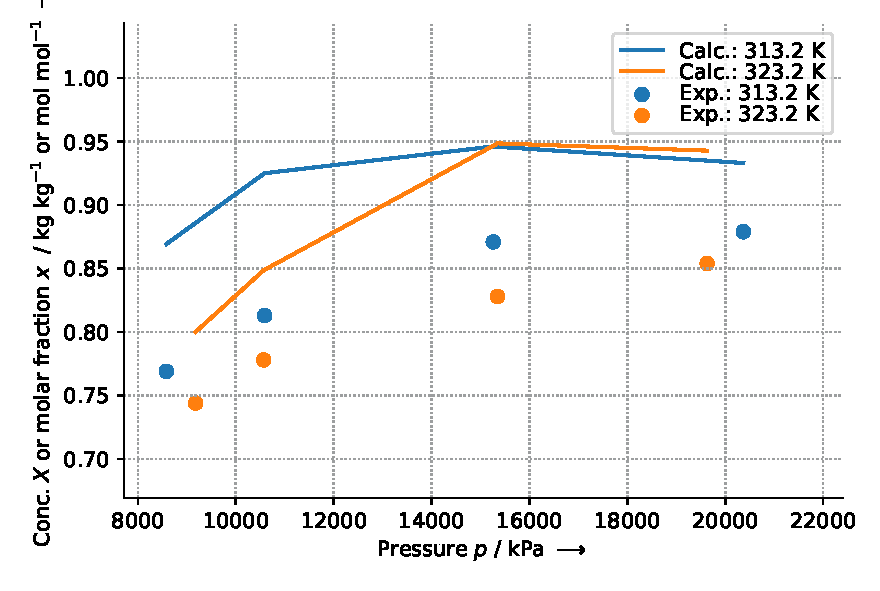
\includegraphics[height=10cm, keepaspectratio]{figs/abs/abs_CarbonDioxide_ionic_liquid_[N4,1,1,1][NTf2]_MixingRule_2.pdf}}
\end{figure}
%

To generate the figure, the following refrigerant functions were selected:
\begin{itemize}
\item Vapor pressure: VaporPressure\_EoS1 - ID 1
\item Saturated liquid density: SaturatedLiquidDensity\_EoS1 - ID 1
\end{itemize}

The uncertainity of the experimental data is:
\begin{itemize}
\item Data source $\,\to\,$ Data was taken from table
\item Pressure, absolute, in $\si{\pascal}$ $\,\to\,$ 7.00E+03
\item Temperature, absolute, in $\si{\kelvin}$ $\,\to\,$ 0.1
\end{itemize}

The mean absolute percentage error (MAPE) between the experimental and calculated data results in 10.4\%.
\FloatBarrier
\newpage
%%%%%%%%%%%%%%%%%%%%%%%%%%%%%%%%%%%%%%%%%%%%%%%%%%%%%%%%%%%%%%%%%%%%%%%%%%%%%%%
